%% Customizações do abnTeX2 (http://www.abntex.net.br) para o Instituto de Matemática,
%% Estatística e Computação Científica da Universidade Estadual de Campinas (IMECC-UNICAMP)
%%
%% This work may be distributed and/or modified under the conditions of the LaTeX Project
%% Public License, either version 1.3 of this license or (at your option) any later version.
%% The latest version of this license is in http://www.latex-project.org/lppl.txt and version
%% 1.3 or later is part of all distributions of LaTeX version 2005/12/01 or later.
%%
%% This work has the LPPL maintenance status `maintained'.
%% 
%% The Current Maintainer of this work is Fábio Rodrigues Silva, gfabinhomat@gmail.com
%%
%% Further information about abnTeX2 are available on http://www.abntex.net.br
%%
\documentclass[
	oldfontcommands,
	% -- opções de customização --
	%sumario=tradicional,
	sumario=abnt-6027-2012,
	% -- opções da classe memoir --
	12pt,			% tamanho da fonte
	openright,		% capítulos começam em pág ímpar (insere página vazia caso preciso)
	oneside,		% para impressão em verso e anverso. Oposto a 'oneside'
	a4paper,		% tamanho do papel. 
	% -- opções da classe abntex2 --
	%chapter=TITLE,		% títulos de capítulos convertidos em letras maiúsculas
	%section=TITLE,		% títulos de seções convertidos em letras maiúsculas
	%subsection=TITLE,	% títulos de subseções convertidos em letras maiúsculas
	%subsubsection=TITLE,	% títulos de subsubseções convertidos em letras maiúsculas
	% -- opções do pacote babel --
	english,		% idioma adicional para hifenização
	brazil			% o último idioma é o principal do documento
	]{imecc-unicamp}
% ----------------------------------------------------------
% PACOTES ESSENCIAIS
% Aqui você pode adicionar seus pacotes específicos para uso em seu trabalho.
% Em PACOTES PESSOAIS insira os pacotes que desejar.
% ----------------------------------------------------------
% PACOTES BÁSICOS (ESSENCIAIS AO MODELO)
\usepackage{lmodern}			% Usa a fonte Latin Modern
\usepackage[T1]{fontenc}		% Selecao de codigos de fonte.
\usepackage[utf8]{inputenc}		% Codificacao do documento (conversão automática dos acentos)
\usepackage{lastpage}			% Usado pela Ficha catalográfica
\usepackage{indentfirst}		% Indenta o primeiro parágrafo de cada seção.
\usepackage{color,xcolor}		% Controle das cores
\usepackage{graphicx}			% Inclusão de gráficos
\usepackage{microtype} 			% para melhorias de justificação

\usepackage{float}
% ----------------------------------------------------------
% ----------------------------------------------------------
% PACOTES PARA GLOSSÁRIO
\usepackage[subentrycounter,seeautonumberlist,nonumberlist=true]{glossaries}
% para usar o xindy ao invés do makeindex:
%\usepackage[xindy={language=portuguese},subentrycounter,seeautonumberlist,nonumberlist=true]{glossaries}
% ----------------------------------------------------------
% ----------------------------------------------------------
% PACOTES DE CITAÇÕES (PRINCIPAIS PACOTES DO MODELO)
\usepackage[brazilian]{backref}		% Paginas com as citações na bibl
\usepackage[alf,
	    abnt-repeated-author-omit=yes,
	    abnt-etal-list=0]{abntex2cite}		% Citações padrão ABNT
% É possível utilizar o sistema numérico de chamada, alterando a opção 'alf' para 'num'.
% Outros estilos bibliográficos podem ser usados. Se este for o caso, comente o pacote acima
% e utilize, por exemplo, o comando abaixo
% \bibliographystyle{acm}
% Consulte outros estilos de bibliografia consultando o manual de estilos bibliográficos do
% BibTeX em 'http://www.bibtex.org/'
% ----------------------------------------------------------
% ----------------------------------------------------------
% PACOTES ADICIONAIS (usados apenas no âmbito do Modelo Canônico do abnteX2)
\usepackage{lipsum}			% para geração de dummy text
% ----------------------------------------------------------
% ----------------------------------------------------------
% PACOTES PESSOAIS (USADOS PELO AUTOR -- acrescente aqui seus pacotes)
% ----------------------------------------------------------
\usepackage[portuguese,onelanguage]{algorithm2e}	% para inserir algoritmos (longend,vlined)
% \usepackage{amsbsy}			% para símbolos matemáticos em negrito
% \usepackage{amscd}			% para diagramas
% \usepackage{amsfonts}			% fontes AMS
% \usepackage{amsmath}			% facilidades matemáticas
% \usepackage{amssymb}			% para os símbolos mais antigos
% \usepackage{amstext}			% para fragmentos tipo texto em modo matemático
\usepackage{amsthm}			% para teoremas
\usepackage{hyperref}			% Amplo suporte para hipertexto em LaTeX
\usepackage{cleveref}			% Referência cruzada inteligente
\usepackage{dsfont}			% para o estilo de conjuntos de números $\mathds{R}$
% \usepackage{ifthen}			% comandos de condição em LaTeX
\usepackage{listings}           	% para inserir códigos de outras linguagens de programação
% \usepackage{lscape}             	% para imprimir alguma página no formato paisagem
\usepackage{mathabx}			% conjunto de simbolos matemáticos
% \usepackage{mathrsfs}			% suporte para fontes RSFS
% \usepackage{pdfpages}           	% para inserir páginas PDF no texto

% \usepackage{verbatim}
% ----------------------------------------------------------
% ----------------------------------------------------------
% ----------------------------------------------------------
% INFORMAÇÕES E DADOS PARA CAPA E FOLHA DE ROSTO
% ----------------------------------------------------------
% Os comandos abaixo devem ser preenchidos em língua PORTUGUESA
\titulo{Desenvolvimento de testes diagnóstico para HPV-16 a partir da modelagem por IA de variantes nas oncoproteínas E6/E7 ao interagir com p53 e p16INK4a}
\tipotrabalho{Relatório parcial de Iniciação Científica}
% \tipotrabalho{Tese}
% \curso{Estatística}
% \curso{Matemática}
% \curso{Matemática Aplicada}
\curso{Programa de Desenvolvimento Tecnológico e Inovação (PIBIT 2025-2026)}
% \curso{}  % Se for aluno do PROFMAT
% ----------------------------------------------------------
% ----------------------------------------------------------
% Os comandos abaixo devem ser preenchidos na língua DO TRABALHO
% ---
% Se autor do sexo MASCULINO
% \autor{Nome Completo do Aluno}
% \titulacao{Mestre}
% \titulacao{Doutor}
% ---
% Se autor do sexo FEMININO, descomente e preencha os campos abaixo
\autor[autora]{Beatriz Souza de Oliveira}
\titulacao{Graduando em Medicina}
% \titulacao{Doutora}
% ---
% Se orientador/coorientador do sexo MASCULINO
% \orientador{Nome Completo do Orientador}
% \coorientador{Nome Completo do Coorientador}
% ---
% Se orientador/coorientador do sexo FEMININO, descomente e preencha os campos abaixo (exceto se o trabalho for em inglês)
\orientador[Orientador]{Profº Dr. Toni Ricardo Martins}
% ---
\data{2025}
% ---
% Se seu trabalho for em língua NÃO portuguesa, descomente e preencha os campos abaixo na lingua DO TRABALHO
% \setboolean{ABNTEXotherlanguage}{true}
% \titulootherlang{Title of your Academic Work:\\ master thesis or phd thesis}
% \cursootherlang{Statistics}
% \cursootherlang{Mathematics}
% \cursootherlang{Applied Mathematics}
% \cursootherlang{Computational and Applied Mathematics}
% \typework{Dissertation}
% \typework{Thesis}
% \titulation{Master}
% \titulation{Doctor}
% ---
% No caso de Cotutela Internacional de Tese, descomente e preencha os campos abaixo
% \setboolean{ABNTEXcotutela}{true}
% \universidadecotutela{NAME OF THE UNIVERSITY}
% \paiscotutela{COUNTRY}
% ----------------------------------------------------------
% ----------------------------------------------------------
% ----------------------------------------------------------
% CONFIGURAÇÕES GERAIS
% As configurações gerais são colocadas aqui, como novos comandos para o corpo do texto,
% informações de bookmark para o PDF, tamanho de parágrafos, entre outros.

% ----------------------------------------------------------
% Configurações do pacote BACKREF
% ----------------------------------------------------------
% Usado sem a opção hyperpageref de backref
\renewcommand{\backrefpagesname}{Citado na(s) página(s):~}
% Texto padrão antes do número das páginas
\renewcommand{\backref}{}
% Define os textos da citação
\renewcommand*{\backrefalt}[4]{
	\ifcase #1 %
		Nenhuma citação no texto.%
	\or
		Citado na página #2.%
	\else
		Citado #1 vezes nas páginas #2.%
	\fi}%
% ---

% ----------------------------------------------------------
% \theoremstyle{plain}
\newtheorem{theorem}{Teorema}%[chapter]
\newtheorem{lemma}{Lema}%[chapter]
\providecommand*{\lemmaautorefname}{Lema}
\newtheorem{proposition}{Proposição}%[chapter]
\providecommand*{\propositionautorefname}{Proposição}
\newtheorem{corollary}{Corolário}%[chapter]
\providecommand*{\corollaryautorefname}{Corolário}
\newtheorem{conjecture}{Conjectura}%[chapter]
\providecommand*{\conjectureautorefname}{Conjectura}
\newtheorem{definition}{Definição}%[chapter]
\providecommand*{\definitionautorefname}{Definição}
\newtheorem{notation}{Notação}%[chapter]
\providecommand*{\notationautorefname}{Notação}
\newtheorem{remark}{Observação}%[chapter]
\providecommand*{\remarkautorefname}{Observação}
\newtheorem{example}{Exemplo}%[chapter]
\providecommand*{\exampleautorefname}{Exemplo}
\newtheorem{note}{Nota}%[chapter]
\providecommand*{\noteautorefname}{Nota}
% ----------------------------------------------------------

% ----------------------------------------------------------
% Conjunto de configuracoes para o pacote 'listings'
% ----------------------------------------------------------
\lstset{
  language=C++,
  basicstyle=\ttfamily, 
  keywordstyle=\color{blue}, 
  stringstyle=\color{verde}, 
  commentstyle=\color{red}, 
  extendedchars=true, 
  showspaces=false, 
  showstringspaces=false,
  numbers=left,
  numberstyle=\tiny,
  breaklines=true, 
  backgroundcolor=\color{green!10},
  breakautoindent=true,
  fontadjust=false
}
% ----------------------------------------------------------

% ----------------------------------------------------------
% Informações do PDF
% ----------------------------------------------------------
% Configurações de aparência do PDF final
% ---
% alterando o aspecto da cor azul
\definecolor{blue}{RGB}{41,5,195}
\definecolor{verde}{rgb}{0,0.5,0}
% ---
\makeatletter
\hypersetup{
  %pagebackref=true,
  pdftitle={\@title},
  pdfauthor={\@author},
  pdfsubject={%
    \imprimirtipotrabalho\ apresentada ao Instituto de Matemática, Estatística %
    e Computação Científica da Universidade Estadual de Campinas como parte dos %
    requisitos exigidos para a obtenção do título de \imprimirtitulacao\ em %
    \imprimircurso.
  },
  pdfcreator={LaTeX with unicamp-abnTeX2},
  pdfkeywords={abnt}{latex}{abntex}{abntex2}{trabalho acadêmico},
  colorlinks=true,		% false: boxed links; true: colored links
  linkcolor=blue,		% color of internal links
  citecolor=blue,		% color of links to bibliography
  filecolor=magenta,		% color of file links
  urlcolor=blue,		% color of internet links
  bookmarksdepth=4
}
\makeatother
% ----------------------------------------------------------

% ----------------------------------------------------------
% COMANDOS GLOBAIS
% ----------------------------------------------------------
\everymath{\displaystyle}
% ---
\renewcommand{\sin}{\mathrm{sen}}
\renewcommand{\tan}{\mathrm{tg}}
\renewcommand{\csc}{\mathrm{cossec}}
\renewcommand{\cot}{\mathrm{cotg}}
% ---
\DeclareMathOperator{\posto}{\mathrm{posto}}
\DeclareMathOperator{\conv}{\mathrm{conv}}
\DeclareMathOperator{\diag}{\mathrm{diag}}
\DeclareMathOperator{\argmin}{\mathrm{arg}\min}
\DeclareMathOperator{\argmax}{\mathrm{arg}\max}
% ---
% O tamanho do parágrafo é dado por:
\setlength{\parindent}{2.0cm}
% Controle do espaçamento entre um parágrafo e outro:
\setlength{\parskip}{0.2cm}  % tente também \onelineskip
% ---
% Para que apareça o nome 'Capítulo X' antes do título de cada capítulo
% \chapterstyle{default}
% ----------------------------------------------------------
\newsubfloat{figure}% Allow subfloats in figure environment
\providecommand*{\subfigureautorefname}{Subfigura}
% ----------------------------------------------------------
% ----------------------------------------------------------
% COMPILA O ÍNDICE (OPCIONAL)
\makeindex
% ----------------------------------------------------------
% ----------------------------------------------------------
% CONTÉM TODAS AS ENTRADAS DO GLOSSÁRIO (OPCIONAL)
\input{glossario}
% ----------------------------------------------------------
% -----------------------------------------------------------------------------------------------
% %%%%%%%%%%%%%%%%%%%%%%%%%%%%%%%%%%%%% INÍCIO DO DOCUMENTO %%%%%%%%%%%%%%%%%%%%%%%%%%%%%%%%%%%%%
% -----------------------------------------------------------------------------------------------
\begin{document}
% Seleciona o idioma do documento (conforme pacotes do babel)
\selectlanguage{brazil}
% \selectlanguage{english}
% Retira espaço extra obsoleto entre as frases.
\frenchspacing
% ---------------------------------------------------------------------------------
% %%%%%%%%%%%%%%%%%%%%%%% INÍCIO DOS ELEMENTOS PRÉ-TEXTUAIS %%%%%%%%%%%%%%%%%%%%%%%
% ---------------------------------------------------------------------------------
\pretextual
% ----------------------------------------------------------
% PRIMEIRA FOLHA (OBRIGATÓRIO)
\imprimirprimeirafolha
% ----------------------------------------------------------
% ----------------------------------------------------------
% FOLHA DE ROSTO (OBRIGATÓRIO)
% ---
% Após realizar as correções finais de seu trabalho acadêmico, escaneie a folha de rosto
% devidamente assinada pelo orientador e salve no formato PDF com o nome 'folha-de-rosto.pdf'
% no diretório do seu projeto. Daí substitua a linha do comando '\imprimirfolhaderosto'
% pelas 3 linhas de comando abaixo:
% ---
% \begin{folhaderosto}
%     \includepdf{folha-de-rosto.pdf}
% \end{folhaderosto}
% ---
\imprimirfolhaderosto

% ----------------------------------------------------------
% ----------------------------------------------------------
% FICHA CATALOGRÁFICA (OBRIGATÓRIO)
% ---
% A biblioteca da UNICAMP lhe fornecerá um PDF com a ficha catalográfica definitiva após a defesa
% do trabalho {http://hamal.bc.unicamp.br/catalogonline2/}. Quando estiver com o documento, salve-o
% como PDF no diretório do seu projeto e deixe apenas o comando '\includepdf{ficha-catalografica.pdf}'
% dentro do ambiente abaixo
% ---
\begin{fichacatalografica}
    \begin{center}
	{\ABNTEXchapterfont\large A ficha catalográfica será fornecida pela biblioteca}
    \end{center}
%     \includepdf{ficha-catalografica.pdf}
\end{fichacatalografica}
% ----------------------------------------------------------
% ----------------------------------------------------------
% FOLHA DE APROVAÇÃO (OBRIGATÓRIO)
% ---
% A folha de aprovação será fornecida pela secretaria de pós-graduação. Após recebê-la, escaneie a folha
% salvando em PDF no diretório do seu projeto com o nome 'folhadeaprovacao.pdf' e deixe apenas o comando
% '\includepdf{folhadeaprovacao.pdf}' dentro do ambiente abaixo
% ---
% ----------------------------------------------------------
% ----------------------------------------------------------
% DEDICATÓRIA (OPCIONAL)
\begin{dedicatoria}
   \vspace*{\fill}
   \centering
   \noindent
   \textit{
      Este trabalho é dedicado às crianças adultas que,\\
      quando pequenas, sonharam em se tornar cientistas.
   }
   \vspace*{\fill}
\end{dedicatoria}
% ----------------------------------------------------------
% ----------------------------------------------------------
% AGRADECIMENTOS (OPCIONAL)
\begin{agradecimentos}
Sou grato a Deus por ser minha maior força todos os dias, e ser a razão do meu existir. 

\end{agradecimentos}
% ----------------------------------------------------------
% ----------------------------------------------------------
% EPÍGRAFE (OPCIONAL)
\begin{epigrafe}
    \vspace*{\fill}
    \begin{flushright}
	\textit{``Seja a luz no mundo''
	}
    \end{flushright}
\end{epigrafe}
% ----------------------------------------------------------
% ----------------------------------------------------------
% RESUMOS (OBRIGATÓRIO)
% -------------------------------------------------------------
%  RESUMOS
\setlength{\absparsep}{18pt} % ajusta o espaçamento dos parágrafos do resumo
% -------------------------------------------------------------
% ATENÇÃO: o ambiente 'otherlanguage*' deve ser usado para o resumo que não está na
% língua vernácula do trabalho, com a respectiva opção linguística do pacote 'babel'.
% -------------------------------------------------------------
% resumo em PORTUGUÊS (OBRIGATÓRIO)
\begin{resumo}[Resumo]
 \begin{otherlanguage*}{brazil}

   Em um esforço para combater as alarmantes taxas de incidência e mortalidade por câncer de colo do útero no estado do Amazonas, um cenário de saúde pública agravado por barreiras geográficas que dificultam o diagnóstico precoce, este projeto de pesquisa propõe uma investigação aprofundada das bases moleculares da agressividade do Papilomavírus Humano tipo 16 (HPV-16), o genótipo de maior risco oncogênico e prevalência na região. A pesquisa foca-se em como as mutações específicas do HPV-16, circulantes na população amazonense e no mundo, alteram a estrutura e a função de suas oncoproteínas cruciais, a E6 e a E7, potencializando a sua capacidade de induzir a transformação maligna das células hospedeiras. A metodologia empregará uma abordagem computacional, iniciando com a modelagem tridimensional das oncoproteínas E6 e E7, tanto em sua forma selvagem quanto incorporando as variantes genéticas encontradas no Amazonas e no mundo, utilizando para isso o poder da inteligência artificial através da ferramenta AlphaFold. Em seguida, serão realizadas simulações de docking molecular para predizer a interação dessas oncoproteínas virais com seus alvos celulares primários, a proteína supressora de tumor p53, que é inativada pela E6, além de investigar interações com a proteína p16INK4a, um biomarcador fundamental na gravidade das lesões cervicais ocasionadas pelo câncer de colo de útero. Também será realizado uma dinâmica molecular ao longo de 200 ns, que permitirá observar o comportamento dos complexos ao longo do tempo. Além disso, serão  propostos anticorpos neutralizantes do vírus e regiões de epítopos antigênicos, bem como sequência de primers para o diagnóstico. Ao fim,  as sequências de proteínas, epítopos e primers encontradas serão disponibilizadas publicamente ao término deste trabalho no Github, o que possibilitará a síntese, purificação e a implementação dos testes diagnósticos num próximo trabalho.

    \textbf{Palavras-chave}: HPV-16, Amazonas, bioinformática, IA, docking molecular, dinâmica molecular

 \end{otherlanguage*}
\end{resumo}
% -------------------------------------------------------------
% -------------------------------------------------------------
% resumo em INGLÊS (OBRIGATÓRIO)
\begin{resumo}[Abstract]
 \begin{otherlanguage*}{english}
    This is the english abstract.
    
    \textbf{Keywords}: latex. abntex. text editoration.
 \end{otherlanguage*}
\end{resumo}
% -------------------------------------------------------------
% ----------------------------------------------------------
% ----------------------------------------------------------
% LISTA DE ILUSTRAÇÕES (OPCIONAL)
\pdfbookmark[0]{\listfigurename}{lof}
\listoffigures*
\cleardoublepage
% ----------------------------------------------------------
% ----------------------------------------------------------
% LISTA DE TABELAS (OPCIONAL)
\pdfbookmark[0]{\listtablename}{lot}
\listoftables*
\cleardoublepage
% ----------------------------------------------------------
% ----------------------------------------------------------
% LISTA DE ABREVIATURAS E SIGLAS (OPCIONAL)
\begin{siglas}
  \item[MD] Dinâmica molecular, do inglês "Molecular Dynamics"
  \item[MM-GBSA] Mecânica molecular por Born-generalizado e solvatação apolar, do inglês "Molecular Mechanics - Generalized Born Solvation Apolar"
\end{siglas}

% ----------------------------------------------------------
% ----------------------------------------------------------
% SUMÁRIO (OBRIGATÓRIO)
\pdfbookmark[0]{\contentsname}{toc}
\tableofcontents*
\cleardoublepage
% ----------------------------------------------------------
% ---------------------------------------------------------------------------------
% %%%%%%%%%%%%%%%%%%%%%%%% FIM DOS ELEMENTOS PRÉ-TEXTUAIS %%%%%%%%%%%%%%%%%%%%%%%%
% ---------------------------------------------------------------------------------
% ---------------------------------------------------------------------------------
% %%%%%%%%%%%%%%%%%%%%%%%%% INÍCIO DOS ELEMENTOS TEXTUAIS %%%%%%%%%%%%%%%%%%%%%%%%%
% ---------------------------------------------------------------------------------
\textual
% ----------------------------------------------------------
% INTRODUÇÃO
% ----------------------------------------------------------
% Exemplo de capítulo sem numeração, mas presente no Sumário
\chapter*[Introdução]{Introdução}
\addcontentsline{toc}{chapter}{Introdução}
% ----------------------------------------------------------

O câncer de colo de útero é uma neoplasia maligna do epitélio de revestimento do órgão, considerado um grave problema de saúde pública global, especialmente prevalente em regiões de baixa e média renda. No Brasil,  é o terceiro tipo mais comum de câncer entre as mulheres, excluindo-se os casos de câncer de pele não melanoma. O carcinoma epidermoide é o subtipo mais incidente, correspondendo a 90\% dos casos. A infecção persistente por tipos oncogênicos do Papiloma Vírus Humano (HPV) é responsável por 99\% dos casos de câncer cervical (INCA,2021). Com isso, é uma doença amplamente prevenível graças a intervenções eficazes como a vacinação contra o HPV, e o rastreamento, com destaque para os métodos baseados na detecção do vírus.

Em resposta a essa realidade, a Organização Mundial da Saúde (OMS) estabeleceu em 2020 a Iniciativa Global para a Eliminação do Câncer Cervical. O objetivo é reduzir a incidência para menos de 4 casos por 100.000 mulheres-ano em todos os países. Para atingir essa meta até 2030, a estratégia da OMS foca em três pilares: vacinar 90\% das meninas até os 15 anos, rastrear 70\% das mulheres com um teste de alta performance pelo menos duas vezes até os 45 anos, e tratar 90\% das mulheres diagnosticadas com pré-câncer ou câncer cervical. Para o sucesso da iniciativa, é crucial que haja monitoramento contínuo e aprimorado para identificar lacunas e direcionar as ações (OMS,2020) (ARBYN, et al. 2020).

Apesar dos esforços, a incidência e a mortalidade do câncer de colo de útero ainda estão muito acima da meta da OMS em muitas regiões, especialmente naquelas com menores níveis de desenvolvimento humano, evidenciando marcantes desigualdades geográficas e socioeconômicas. Cidades como Manaus (Amazonas) ainda enfrentam obstáculos substanciais. Apesar da disponibilidade de exames citológicos gratuitos desde 1990 e imunização contra o HPV desde 2013, a capital amazonense mantém uma das maiores incidências de câncer cervical no mundo, refletindo limitações no rastreamento, cobertura vacinal e monitoramento das cepas virais circulantes (TORRES et al, 2021). 

Para mudar esse cenário, a implementação de programas de rastreamento organizados, aliados ao acesso a tratamento acessível e a uma maior cobertura vacinal contra o HPV, será fundamental para reduzir a incidência e a mortalidade nas próximas décadas. É essencial aplicar as novas ferramentas de prevenção e controle de forma criteriosa, considerando o contexto de cada local, e continuar monitorando a doença globalmente, especialmente entre as populações mais vulneráveis, pois os fatores socioeconômicos desempenham um papel crucial nas desigualdades do câncer (SINGH et al, 2023).

Avanços recentes na região incluem a aplicação do teste OncoE6™, voltado para a detecção da oncoproteína E6 do HPV-16 e HPV-18, em populações ribeirinhas e de difícil acesso no Amazonas. Tal abordagem demonstrou-se viável e altamente específica, evidenciando o potencial de inovações capazes de mitigar barreiras logísticas e, ao mesmo tempo, permitir uma cobertura de triagem expandida, um aspecto fundamental para mulheres que, diante de resultados anormais, enfrentam dificuldades para obter acesso à colposcopia e ao tratamento especializado (Torres et al., 2018).
Paralelamente, estudos genômicos locais identificaram mutações missense em genes provenientes de variantes do HPV-16 que circulam especificamente no estado do Amazonas. No gene E6, as mais frequentes observadas foram T7392G (L90V) — leucina por valina (45,5\%), C7377T (H85Y) — histidina por tirosina (39,4\%), e G7187T (Q21H) — glutamina por histidina (39,4\%). No gene E7, foram encontradas: G7810A (G43E) — glicina por glutamato, e A7689G (N29S) — asparagina por serina. (RONDON et al, 2024). Tais alterações podem modificar propriedades estruturais e funcionais dessas oncoproteínas, impactando diretamente sua interação com genes supressores de tumor, como p53 e p16INK4a.

A ausência de dados estruturais tridimensionais sobre essas variantes locais representa uma importante lacuna científica, com implicações no desenvolvimento de vacinas personalizadas, terapias-alvo e métodos diagnósticos mais precisos. Frente a esse cenário, o presente projeto propõe o uso de tecnologias emergentes de inteligência artificial (IA) - em especial, o software AlphaFold - para modelar, simular e prever interações estruturais das oncoproteínas E6 e E7 mutadas com alvos celulares de importância oncológica. Complementando essa abordagem, serão realizados docking molecular, predição de epítopos antigênicos e análise de interação com anticorpos para clonagem in silico de um potencial teste diagnóstico, além da disponibilização dos dados em uma base pública.
Dessa forma, a presente proposta visa investigar mutações regionais e mundiais do HPV-16 associadas ao câncer cervical, empregando tecnologias computacionais avançadas aplicadas à modelagem molecular e simulações biofísicas, com ênfase no desenvolvimento de soluções inovadoras para o diagnóstico e prevenção da doença, especialmente adaptados à realidade epidemiológica da região amazônica. 
Com forte potencial de inovação translacional, o projeto utiliza da bioinformática para transformar dados genéticos locais em aplicações biomédicas relevantes e compactuam com os objetivos da OMS para erradicação do câncer de colo cervical até 2030. 


\section{Via da beta-catenina}

A via Wnt desempenha papel central na regulação da proliferação e diferenciação celular, estando frequentemente desregulada no câncer colorretal (CCR) \cite{Liu2022}. A $\beta$‑catenina é o principal efetor dessa via, atuando como cofator transcricional ao interagir com proteínas como TCF4, BCL9 e LEF1². Essas interações promovem a ativação de genes relacionados à progressão tumoral e resistência terapêutica³. O bloqueio seletivo dessas interfaces
desponta como estratégia promissora para o desenvolvimento de novas terapias‑alvo no CCR, especialmente por meio de abordagens in silico, que permitem prever afinidades e potenciais pontos de intervenção \cite{Liu2022}. Este estudo comparou a estabilidade e a afinidade de ligação dos complexos $\beta$‑catenina/TCF4, $\beta$‑catenina/BCL9 e $\beta$‑catenina/LEF1, buscando identificar possíveis alvos terapêuticos na via Wnt.
% ----------------------------------------------------------
% DESENVOLVIMENTO
% \part{Preparação da pesquisa}
% \include{capitulo1}
% \include{capitulo2}
% \part{Referenciais teóricos}
% \include{capitulo3}
% \include{capitulo4}
% \include{capitulo5}
% \part{Resultados}
% \include{capitulo6}
% \include{capitulo7}
% --------------------
% INÍCIO DOS EXEMPLOS
% --------------------
% No âmbito do Modelo Canônico, os comandos a seguir apresentam um sucinto resumo de como
% esta classe pode ser usada. Oriente a construção do seu trabalho com base nestes comandos.
% ---
\chapter{Objetivos}

Investigar como mutações identificadas no estado do Amazonas e no mundo para o HPV-16 podem interferir no reconhecimento de proteínas supressoras de tumor.

\section{Objetivos específicos}

\begin{enumerate}
    \item Modelar a estrutura tridimensional das proteínas E6 e E7 usando o AlphaFold tanto para forma ausente de mutações quanto para as mutações L90V, H85Y e Q21H para E6. Além da inserção das mutações G43E e G43E para E7 encontradas no Amazonas, e outras a nível mundial;

    \item Realizar o docking molecular usando o AlphaFold com proteínas supressores de tumor p53 e P16INK4a;

    \item Simular a dinâmica molecular ao longo de 200 ns (nanossegundos) da interação do complexo E6/E7 com as proteínas supressoras;

    \item Predição de epítopos antigênicos e primers dos segmentos E6 e E7 e avaliar a interação com anticorpos neutralizantes para o desenvolvimento de novos diagnósticos rápidos para HPV-16;

    \item Disponibilizar publicamente os dados obtidos no Github, criando uma base de dados acessível.
\end{enumerate}

\part{Materiais e Métodos}

% ----------------------------------------------------------
% Este capítulo, utilizado por diferentes exemplos do abnTeX2, ilustra o uso de
% comandos do abnTeX2 e de LaTeX.
% ----------------------------------------------------------

\chapter{Materiais e Métodos}\label{cap_exemplos}

\section{Modelagem estrutural das mutações}

O sequenciamento genético da forma ausente de mutações (wild-type) será obtida pela plataforma NCBI pelo código NC\_001526 referente ao HPV-16, onde a transcrição para o segmento E6 e E7 já é fornecida. A partir das mutações já descobertas e publicadas na literatura, entre estas a H85Y e  será feita a predição estrutural por um algoritmo de deep-learning, uma técnica avançada de IA utilizando o servidor do AlphaFold (https://alphafoldserver.com/). Os dados de entrada consistirão basicamente na sequência de aminoácidos do segmento E6 e E7, ao interagir com proteínas supressores de tumor, dentre estas p53. 

As estruturas foram validadas pelo mapa de contato gerado na própria ferramenta fornecendo um score e também pela plataforma MolProbity. Além disso, serão empregados estruturas já resolvidas experimentalmente por técnicas cristalográficas depositadas na base de dados Protein Data Bank, incluindo a interação p53-E6-E6AP sob o código de PDB ID: 4XR8 (Zapien et al, 2016). Além disso, será analisado como os anticorpos neutralizante V5 e U4 agem com a proteína L1 do capsídeo do HPV-16 sob o código PDB ID: 6BT3 (Guan et al, 2017).

\section{Predição de epítopos antigênicos}

A predição de epítopos antigênicos tanto para os segmentos L1/L2 quanto E6/E7 será realizada com base nas mutações detectadas no Amazonas, no Brasil e no mundo. Será empregado a ferramenta IEDB-MHC-I (https://www.iedb.org/) bem como IEDB-T-Cell que faz uso de redes neurais artificiais (VITA et al, 2025), um subtipo de IA, em diferentes alelos HLA. Os epítopos gerados serão modelados usando o AlphaFold e posteriormente feito o docking com receptor de células-T e Toll-like receptor II (TLR2) para avaliação da imunogenicidade.

\section{Docking molecular do tipo proteína-proteína}

As sequências de aminoácidos de referência (wild-type) para as oncoproteínas E6 e E7 do HPV-16 foram extraídas do genoma de referência depositado na plataforma NCBI (GenBank ID: NC\_001526). As sequências foram então modificadas in silico para introduzir as mutações de sentido trocado (missense) de interesse, previamente identificadas em pacientes do estado do Amazonas, no Brasil e no mundo.

A predição da estrutura tridimensional das proteínas, tanto na forma wild-type quanto mutante, foi realizada utilizando o AlphaFold server, um algoritmo de deep learning de alta precisão. A qualidade dos modelos gerados foi rigorosamente avaliada por dois métodos complementares: Análise de Confiança Interna, utilizando do escore pLDDT (predicted Local Distance Difference Test) gerado pelo próprio AlphaFold, o qual estima a confiabilidade da predição por resíduo; e Validação Geométrica Externa com a submissão dos modelos à plataforma MolProbity para análise da qualidade estereoquímica, incluindo ângulos da cadeia principal (Mapa de Ramachandran) e contatos estéreis. 

Para fins comparativos e de validação dos modos de interação, foram empregadas estruturas resolvidas experimentalmente e depositadas no Protein Data Bank (PDB). Isso incluiu o complexo p53-E6-Ubiquitina (PDB ID: 4XR8). A metodologia pode ser resumida conforme a Figura 1.


Para avaliar o impacto das mutações na afinidade de interação, bem como a ligação dos epítopos preditos, foram realizadas simulações de docking proteína-proteína. Realizou-se o docking na ferramenta PIPER integrada ao software Schrodinger Maestro 2021-2 em sistema operacional Linux. A afinidade de interação foi quantificada em termos de energia livre de ligação ($\Delta G$, em kcal/mol).

\begin{figure}[H]
    \centering
    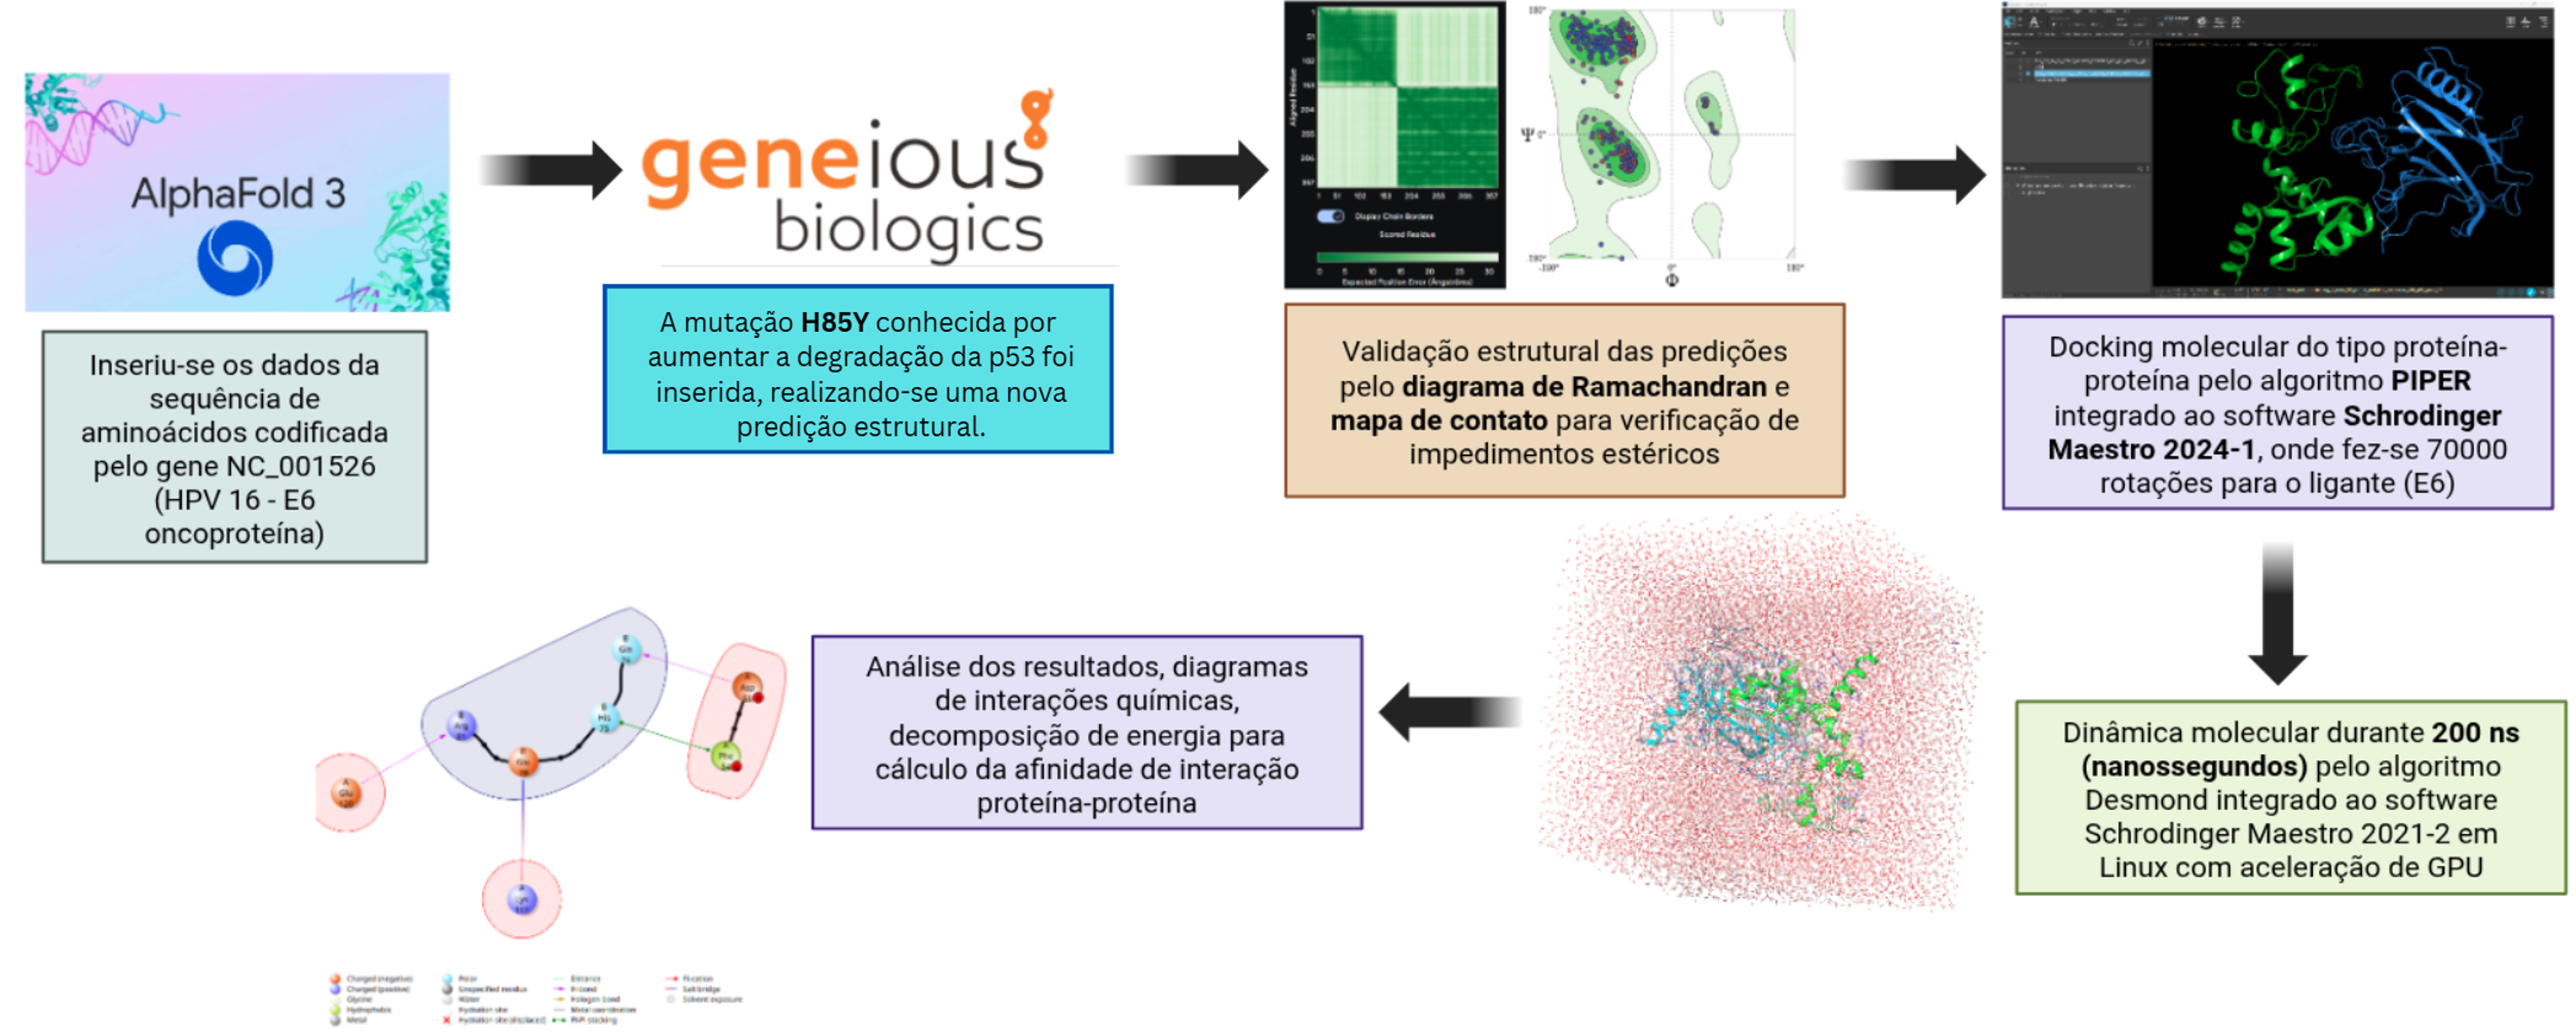
\includegraphics[width=1\linewidth]{Figuras/fluxograma_metodologia.png}
    \caption{Diagrama da metodologia computacional empregada.}
    \label{fig:enter-label}
\end{figure}

\section{Dinâmica molecular na avaliação da estabilidade estrutural}
A partir dos complexos obtidos no docking molecular foi realizado a dinâmica molecular ao longo de 200 ns no software Schrodinger Maestro 2022-1 (Schrödinger, 2022) na sua versão de Linux Ubuntu 24.10 mediante o módulo Desmond com aceleração de GPU RTX 3050. Os parâmetros da simulação foram mantidos a temperatura e pressão constante de 300 K e 1 atm mediante os termostatos de Langevin e barostato de Nosé-Hoover sob o ensemble NPT (número de partículas constante, pressão e temperatura constante). O modelo teórico para as moléculas de água foi o TIP3P com uma caixa de solvatação de geometria cúbica em torno dos complexos. As análises feitas de estabilidade foi principalmente o RMSD (root-mean square deviation) e RMSF (root-mean square fluctuation) ao longo do tempo. Em seguida, foi feito a decomposição de energia MM-GBSA a partir dos últimos 20 ns de simulação para estimativa da afinidade de interação ($\Delta G_{binding}$).

\section{Design de primers para os oncogenes E6/E7}

Serão desenhados um par de primers (Forward e Reverse) que amplifique de forma específica e eficiente uma região conservada dos oncogenes E6 ou E7 do HPV-16, que são os alvos mais comuns para diagnóstico de alto risco. Utilizando-se o software Geneious 11.1.5, fez-se o download do genoma completo do Papilomavírus humano tipo 16 a partir do código de acesso de referência no NCBI GenBank NC\_001526. Após importar, será visualizado a sequência circular do genoma do HPV-16 com suas anotações (genes como E6, E7, L1, L2, etc.) A maioria das reações de PCR (especialmente qPCR), um produto (amplicon) entre 100 e 300 pares de base (pb) é considerado ideal, onde o gene E6/E7 foram selecionado nos quais os primers deverão se anelar. Será utilizado o algoritmo Primer3, que é o padrão-ouro para desenho de primers (UNTERGASSER et al., 2012).

\section{Clonagem e expressão recombinante dos epítopos}

A ferramenta de adaptação de Códons desenvolvida em Java (JCAT) (http://www.prodoric.de/JCat) será utilizada para tradução reversa e otimização de códons de vacinas candidatas projetadas. A otimização de códons será executada para expressar a construção vacinal multiepítopo do vírus HPV-16 em E. coli (cepa K12). Os arquivos de saída serão verificados quanto ao Índice de Adaptação de Códons (IAC) (> 0,8–1,0) e ao conteúdo de GC (30–70\%), para garantir a eficiência transcricional e translacional da construção vacinal projetada. A sequência otimizada de códons resultante das vacinas candidatas será introduzida em sítios específicos. O SnapGene (www.snapgene.com) será finalmente utilizado para inserir a sequência da vacina no vetor de expressão pET-30a(+), entre o sítio de clonagem XhoI e NdeI, obtendo-se os clones finais das vacinas candidatas.

\section{Modelagem da $\beta$-catenina}

As estruturas tridimensionais dos complexos foram modeladas por meio do AlphaFold 3 \cite{Abramson2024} utilizando sequências obtidas no UniProt ($\beta$‑catenina: P35222; TCF4: P15884; BCL9: Q9H1M3; LEF1: Q9NQB0). As interações foram analisadas no PyMOL (Schrödinger, LLC) e avaliadas energeticamente com o servidor PRODIGY \cite{Xue2016}, que fornece valores de energia livre de ligação ($\Delta G$) e constante de dissociação ($K_d$). Foram também
identificados os contatos interfaciais (ICs), classificados em charged–charged, charged–polar, charged–apolar, polar–polar, polar–apolar e apolar–apolar. O perfil de superfície não interfacial (NIS) foi calculado para estimar a proporção de resíduos carregados e apolares.

\chapter{Resultados e Discussões}

Este estudo demonstrou que as mutações encontradas na variante H85Y da oncoproteína E6 do HPV-16 enfraquecem significativamente sua interação com a proteína supressora de tumor p53 em comparação ao wild-type (Figura 2). Essa conclusão é sustentada por uma perda drástica de contatos moleculares: enquanto a forma não mutada do complexo se estabiliza com n ligações de hidrogênio, a variante amazônica mantém apenas n-1 (Figura 3).

\begin{figure}[H]
    \centering
    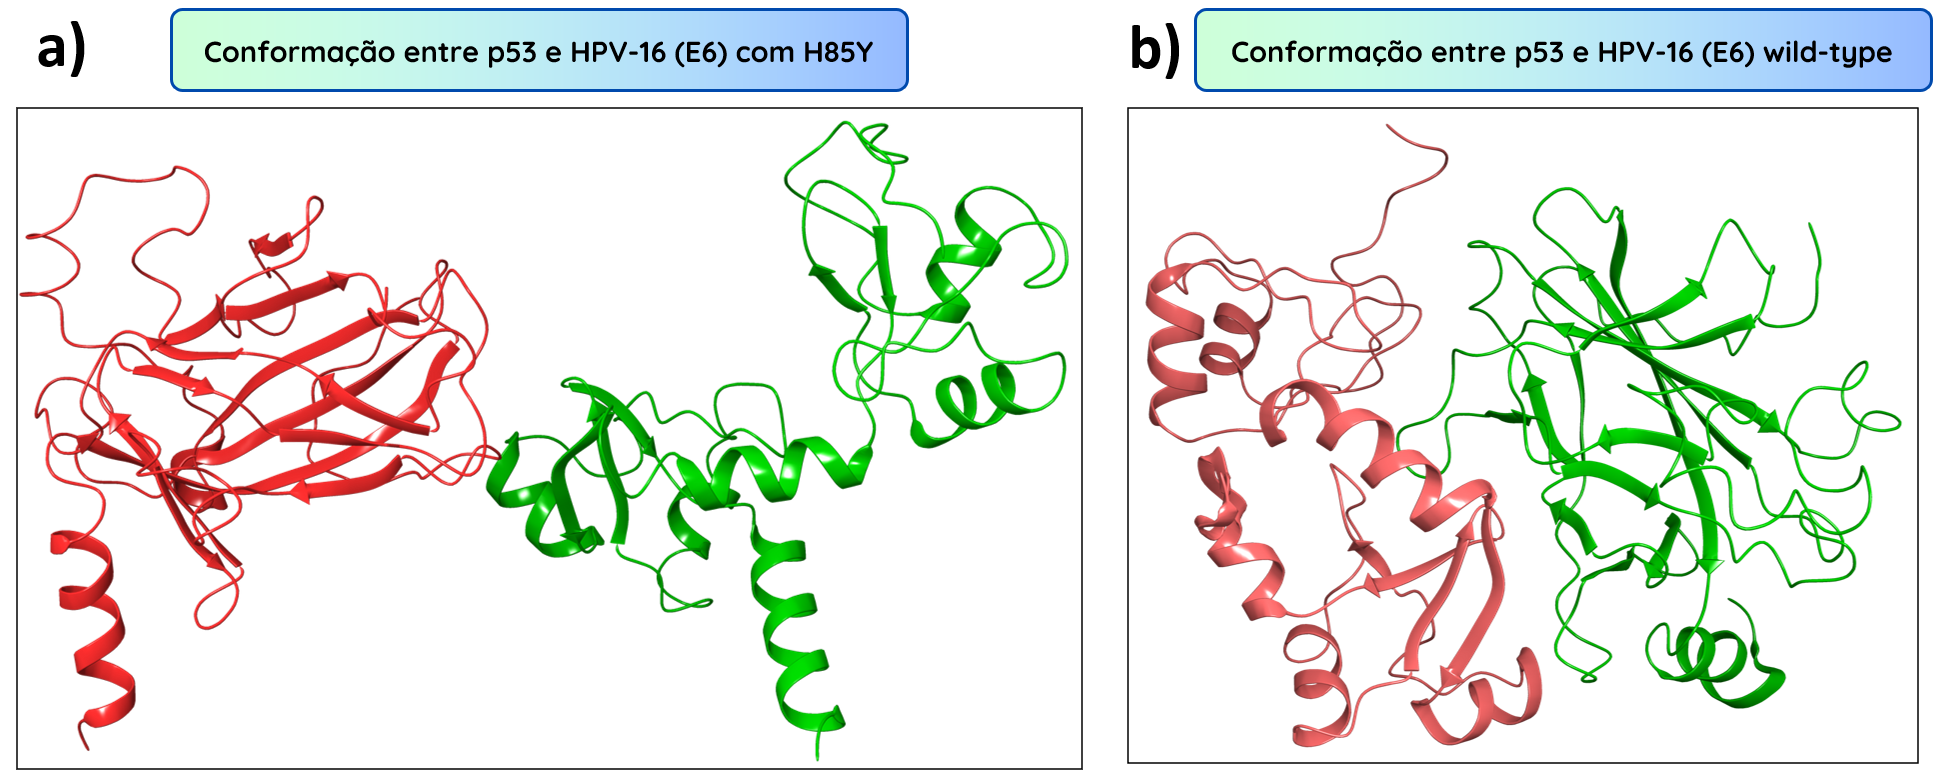
\includegraphics[width=1\linewidth]{Figuras/comparativo_HPV_16_E6_H85_vs_wild_type.png}
    \caption{a) Estrutura tridimensional do frame final após 200 ns de dinâmica molecular da interação entre p53 neutralizando a oncoproteína E6 com a mutação H85Y; b) Estrutura do complexo p53-E6 na forma wild-type, sem mutações; }
    \label{fig:enter-label}
\end{figure}

\begin{figure}[H]
    \centering
    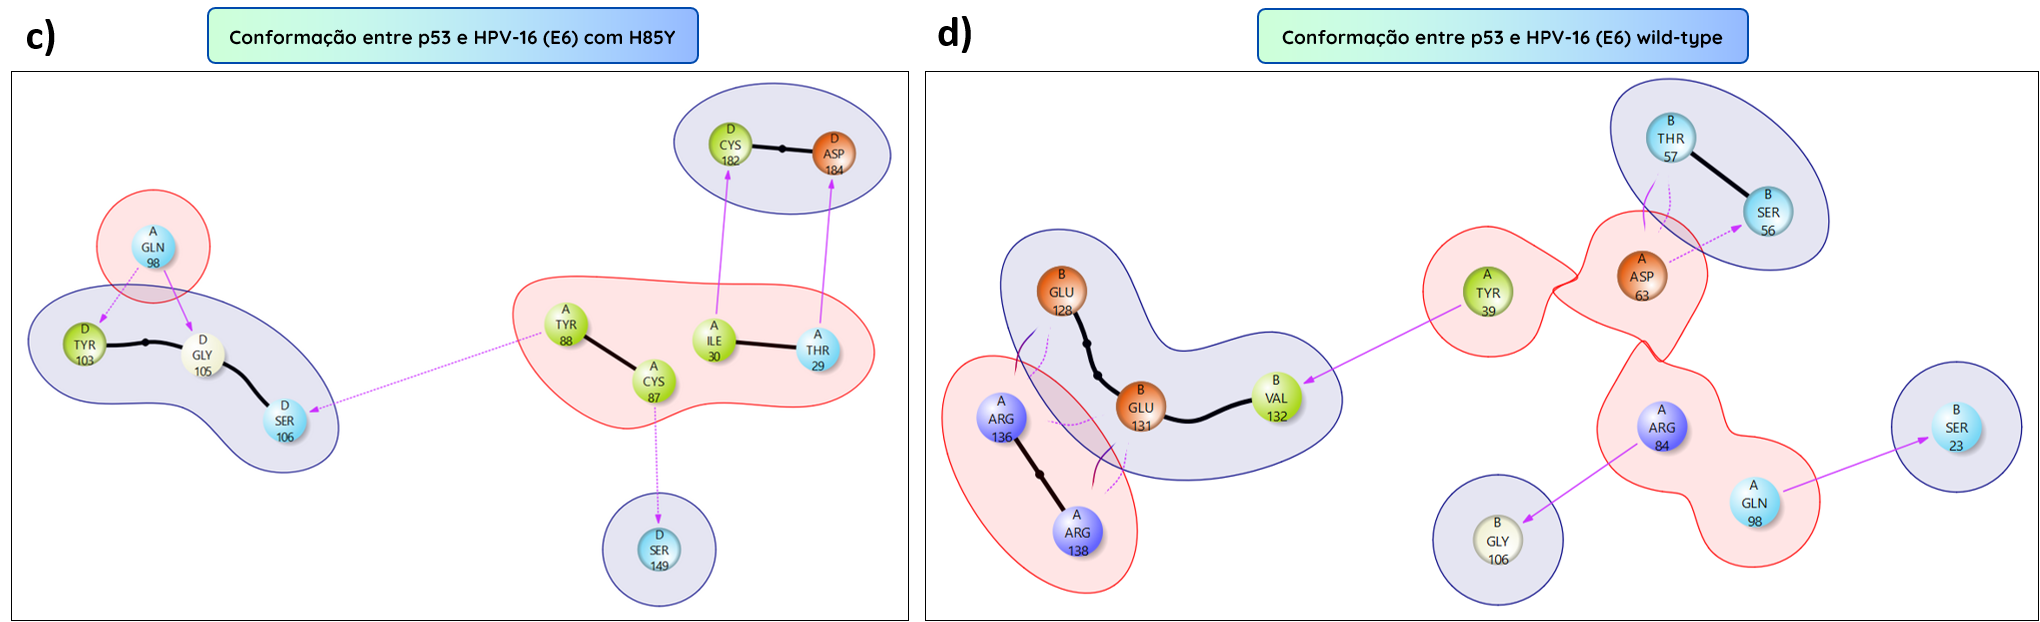
\includegraphics[width=1\linewidth]{Figuras/comparativo_interacoes_HPV_16_E6.png}
    \caption{c) Diagrama de interações para mutação H85Y; d) Diagrama de interações para forma wild-type. }
    \label{fig:enter-label}
\end{figure}


\section{Predição dos epítopos e análise de afinidade}

\begin{table}[H]
    \centering
    \caption{Resultados de afinidade dos epítopos encontrados na interação com receptor de célula T.}
    \begin{tabular}{ccc}
    \hline 
     Sequência    &  $\Delta G$ (kcal/mol)    \\ \hline

    TIHDIILECV  & -42.03 \\
    KLPQLCTEL  & -68. 68 \\ \hline
    \end{tabular}
    \label{tab:my_label}
\end{table}

\section{Predição de miRNA em câncer colorrectal}

\begin{table}[H]
    \centering
    \caption{Resultados de afinidade dos miRNA encontrados na interação com a proteína Argonauta-2.}
    \begin{tabular}{ccc}
    \hline 
     Sequência    &  $\Delta G$ (kcal/mol)    \\ \hline

    mir\_3120\_3p\_2  & -75.14 \\  \hline
    \end{tabular}
    \label{tab:my_label}
\end{table}

\section{Resultado do doking beta-catenina com BCL9, LEF1 e TCF4}

O complexo $\beta$‑Catenina/TCF4 apresentou $\Delta G$ de -26.2 kcal/mol e constante de dissociação ($K_d$) de
$5.9 \times 10^{-20} M$, indicando uma interação de altíssima afinidade. A análise de contatos interfaciais
revelou predominância de interações charged–apolar (95) e charged–polar (49), além de 42
interações charged–charged, demonstrando que a interface é estabilizada por uma combinação de
forças eletrostáticas, hidrofóbicas e de complementaridade estrutural. O perfil de superfície não
interfacial mostrou 23.56\% de resíduos carregados e 43.39\% apolares, sugerindo equilíbrio entre
solubilidade e estabilidade do complexo.

O complexo $\beta$‑Catenina/BCL9 apresentou $\Delta G$ de -37.9 kcal/mol e constante de dissociação
($K_d$) de $1.5 \times 10^{-28} M$, evidenciando uma interação de afinidade ainda mais elevada que a
observada para $\beta$‑catenina/TCF4. A análise de contatos interfaciais indicou predominância
de interações apolar–apolar (136) e charged–apolar (121), complementadas por 48 contatos
charged–charged e 43 charged–polar, configurando uma interface altamente estabilizada
por forças hidrofóbicas e eletrostáticas. O perfil de superfície não interfacial revelou 17.95\% de resíduos carregados e 
51.47\% apolares, reforçando a natureza hidrofóbica dominante do complexo e sua elevada estabilidade conformacional. 
Esses achados destacam o papel crítico de BCL9 como coativador da via Wnt e refletem uma complementaridade estrutural
mais robusta que a observada no complexo $\beta$‑catenina/TCF4.

O complexo $\beta$‑Catenina/LEF1 apresentou $\Delta G$ de -24.0 kcal/mol e constante de dissociação
($K_d$) de $2.4 \times 10^{-18} M$, indicando uma interação de alta afinidade, embora menos intensa do
que as observadas para $\beta$‑catenina/TCF4 e $\beta$‑catenina/BCL9. A análise de contatos
interfaciais revelou predominância de interações charged–apolar (73) e apolar–apolar (59),
além de 42 contatos polar–apolar e 35 charged–charged, sugerindo uma interface
estabilizada principalmente por forças hidrofóbicas, mas com contribuição relevante de
interações eletrostáticas. O perfil de superfície não interfacial apresentou 24.87\% de
resíduos carregados e 43.05\% apolares, indicando equilíbrio entre solubilidade e
estabilidade estrutural. Esses dados reforçam o papel de LEF1 como cofator relevante da
via Wnt, ainda que sua afinidade com a $\beta$‑catenina se apresente inferior àquela observada
para BCL9.

A Tabela 1 resume os resultados obtidos. O complexo $\beta$‑catenina/BCL9 apresentou a maior
afinidade ($\Delta G = -37.9 kcal/mol$; $Kd = 1.5 \times 10^{-28} M$), superando $\beta$‑catenina/TCF4 ($\Delta G =
-26.2 kcal/mol$) e $\beta$‑catenina/LEF1 ($\Delta G = -24.0 kcal/mol$).

\begin{table}[H]
    \centering
    \caption{ Parâmetros energéticos e de contatos interfaciais dos complexos $\beta$‑catenina/TCF4, $\beta$‑catenina/BCL9 e $\beta$‑catenina/LEF1.}
    \begin{tabular}{ccc}
    \hline 
     Interação    & $\Delta G$ (kcal/mol)  & $K_d (M)$   \\ \hline

    $\beta$-Catenina / TCF4 & -26.2 & 5.9 $\times$ 10$^{-20}$  \\
    $\beta$-Catenina / BCL9 & -37.9 & 1.5 $\times$ 10$^{-28}$ \\
   $\beta$-Catenina / LEF1 & -24.0 & 2.4 $\times$ 10$^{-18}$  \\ \hline
    \end{tabular}
    \label{tab:my_label}
\end{table}

A análise mostra que a interação $\beta$‑catenina/BCL9 é mais estável e fortemente guiada por
contatos hidrofóbicos (AA e CA), indicando que essa interface é crítica para a manutenção
da sinalização Wnt. Já o complexo $\beta$‑catenina/TCF4 apresentou predominância de
interações eletrostáticas (CC e CP), reforçando seu papel de especificidade na transcrição
gênica. O complexo $\beta$‑catenina/LEF1, com afinidade intermediária, combina contatos
hidrofóbicos e eletrostáticos, sugerindo que pode atuar como regulador adicional, mas
menos dominante que BCL9. Esses achados são consistentes com a literatura, que aponta
BCL9 como um dos principais coativadores da via Wnt em tumores avançados.

Os resultados obtidos permitem uma análise comparativa da afinidade e estabilidade
estrutural dos complexos da $\beta$‑catenina com três parceiros-chave da via Wnt: TCF4, BCL9 e
LEF1.

O complexo $\beta$‑catenina/BCL9 apresentou a maior afinidade ($\Delta G = -37.9 kcal/mol$;
$K_d = 1.5 \times 10^{-28} M$), superando $\beta$‑catenina/TCF4 e $\beta$‑catenina/LEF1.

A elevada contribuição de interações apolar–apolar (136) sugere que BCL9 exerce
papel crítico na estabilização prolongada do complexo.

Já $\beta$‑catenina/TCF4, apesar de menor $\Delta G$, mantém alta relevância funcional devido
à sua predominância de interações eletrostáticas (charged–polar e
charged–charged), o que favorece a especificidade no reconhecimento.

$\beta$‑catenina/LEF1 apresentou afinidade intermediária, com equilíbrio entre contatos
hidrofóbicos e eletrostáticos, reforçando sua função como modulador, mas
possivelmente com papel menos dominante que BCL9 e TCF4.
Implicações funcionais:

O predomínio de interações hidrofóbicas no complexo $\beta$‑catenina/BCL9 sugere que
a sua interrupção poderia desestabilizar significativamente a sinalização Wnt, sendo
um alvo estratégico.

O complexo $\beta$‑catenina/TCF4, essencial para a transcrição gênica, permanece como
alvo clássico, mas pode demandar abordagens que preservem a seletividade para
evitar toxicidade.

LEF1, embora com afinidade menor, pode atuar em redundância com TCF4,
sugerindo que terapias combinadas visando múltiplas interfaces podem ser mais
eficazes.

A identificação de $\Delta G$ e perfis de interação fornece subsídios para o
desenvolvimento de peptídeos miméticos ou pequenas moléculas inibidoras capazes
de competir com TCF4, BCL9 ou LEF1 pela ligação à $\beta$‑catenina.

O bloqueio específico da interface $\beta$‑catenina/BCL9 surge como promissora
estratégia, dada sua afinidade superior, podendo resultar em maior supressão da via
Wnt em contextos tumorais. No entanto, o equilíbrio observado em LEF1 e TCF4 sugere que abordagens
multitarget podem prevenir mecanismos de escape celular. Estudos futuros devem avaliar não apenas a afinidade estática, mas também a dinâmica conformacional e a viabilidade farmacológica de candidatos, ampliando o potencial de translação clínica dos achados.
% ---
% --------------------
% FIM DOS EXEMPLOS
% --------------------
% ----------------------------------------------------------
% CONSIDERAÇÕES FINAIS
% Finaliza a parte no bookmark do PDF para que se inicie o
% bookmark na raiz e adiciona espaço de parte no Sumário
\phantompart
\chapter{Considerações Finais}

O presente estudo comparativo demonstrou que a interface $\beta$‑catenina/BCL9 apresenta
maior estabilidade e afinidade do que os complexos $\beta$‑catenina/TCF4 e $\beta$‑catenina/LEF1,
reforçando seu potencial como alvo terapêutico prioritário no câncer colorretal. A
abordagem in silico permitiu caracterizar detalhadamente os perfis de interação, sugerindo
que o desenvolvimento de peptídeos miméticos ou inibidores específicos dessa interface
pode constituir uma estratégia promissora para a supressão da via Wnt. Futuras
investigações devem incluir simulações dinâmicas e triagem de candidatos farmacológicos
para validar a viabilidade clínica desses achados.

As mutações encontradas para o vírus HPV-16, especialmente a H85Y comprometem a integridade estrutural do complexo E6-p53. Os picos de RMSD na dinâmica molecular foram maiores para wild-type, o que induziu maiores alterações conformacionais e inibição pela p53. Dessa forma, os resultados fornecem uma base molecular para a hipótese de que pacientes infectados com esta variante possam apresentar desfechos clínicos distintos. 



% ----------------------------------------------------------
% ---------------------------------------------------------------------------------
% %%%%%%%%%%%%%%%%%%%%%%%%%% FIM DOS ELEMENTOS TEXTUAIS %%%%%%%%%%%%%%%%%%%%%%%%%%
% ---------------------------------------------------------------------------------
% ---------------------------------------------------------------------------------
% %%%%%%%%%%%%%%%%%%%%%%% INÍCIO DOS ELEMENTOS PÓS-TEXTUAIS %%%%%%%%%%%%%%%%%%%%%%%
% ---------------------------------------------------------------------------------
% ----------------------------------------------------------
\postextual
% ----------------------------------------------------------
% ----------------------------------------------------------
% REFERÊNCIAS
\bibliography{Referencias}

% ----------------------------------------------------------
%-----------------------------------------------------------
% INDICE REMISSIVO
%-----------------------------------------------------------
\phantompart
\printindex
%-----------------------------------------------------------
% ---------------------------------------------------------------------------------
% %%%%%%%%%%%%%%%%%%%%%%%%%% FIM DOS ELEMENTOS TEXTUAIS %%%%%%%%%%%%%%%%%%%%%%%%%%
% ----------------------------------------------------------------------------------
% -----------------------------------------------------------------------------------------------
% %%%%%%%%%%%%%%%%%%%%%%%%%%%%%%%%%%%%%% FIM DO DOCUMENTO %%%%%%%%%%%%%%%%%%%%%%%%%%%%%%%%%%%%%%
% -----------------------------------------------------------------------------------------------
\end{document}